\chapter{Boules de feu, référentiels et quadrivecteurs}

Nous partons d’une question laissée en suspens après la discussion des collisions à haute énergie. La collision de deux noyaux lourds crée un objet qui évolue violemment, et non un trou noir astronomique au repos. Que peut donc signifier décrire la collision au moyen d’un horizon ? La réponse passe par une représentation en cinq dimensions de la matière fortement couplée, par quelques questions pratiques sur les accélérateurs, puis nous ramène à la géométrie de la relativité restreinte. À la fin, vitesse et quantité de mouvement sont devenues des quadrivecteurs, et l’énergie a pris place aux côtés des trois composantes de la quantité de mouvement.

\section{Une boule de feu dans une cinquième dimension}

\begin{classroomqa}\audiencequestion{L’objet produit par la collision est instable et change de forme. Comment peut-on appeler trou noir un objet aussi complexe ?}\lecturerresponse{Imaginons une cinquième direction spatiale qui s’étend entre un plancher et un plafond. La gravité dans cette direction attire les excitations vers le plancher. La collision y dépose une masse d’énergie chaude ; celle-ci s’étale et change de forme, mais elle peut tout de même posséder un horizon, une température et une entropie.}\end{classroomqa}

Imaginons des particules — ou, de façon plus imagée, de petites cordes — qui se déplacent dans ce monde à cinq dimensions. Les excitations qui tombent vers le plancher apparaissent en quatre dimensions sous la forme de hadrons : protons, neutrons, mésons et autres objets composites étendus. Celles qui restent près du plafond paraissent plus élémentaires. La position verticale fournit donc une manière géométrique d’encoder l’échelle : le plancher représente le régime hadronique à longue distance, tandis que le plafond représente les degrés de liberté à courte distance.

Lorsque deux hadrons entrent en collision, deux objets proches du plancher se heurtent et produisent une grande gerbe d’énergie. Le résultat n’est pas un corps rigide. C’est une masse chaude dotée d’un horizon, une sorte de flaque dans le champ gravitationnel à cinq dimensions. Ce n’est ni un trou noir astronomique dans l’espace ordinaire à quatre dimensions, ni un trou noir à l’échelle de Planck fixé au plafond. C’est la description gravitationnelle de la boule de feu fortement couplée près du plancher.

À haute énergie, les noyaux incidents sont contractés par effet Lorentz en fines crêpes. Ils entrent en collision, déposent leur énergie dans une petite région et produisent un fluide qui évolue vers l’équilibre. Sa faible viscosité était l’une des propriétés surprenantes du plasma de quarks--gluons. Dans la description à cinq dimensions, cette même évolution correspond à la relaxation d’un horizon déformé.

\begin{figure}[H]\centering
\includegraphics[width=0.82\textwidth]{lecture_05_figure_01.png}\caption{Représentation de la cinquième dimension par un plancher et un plafond. Après la collision, la masse centrale dotée d’un horizon s’étale le long du plancher.}\lectureframe{00:04:22}\end{figure}

Un horizon ne persiste pas éternellement. Le rayonnement de Hawking emporte de l’énergie ; dans la description à quatre dimensions, ce rayonnement est la gerbe de hadrons ordinaires qui émergent de la collision. Dans ce langage, les milliers de traces d’un événement détecté sont les particules émises par le trou noir dual, comme si elles en avaient bouilli.

\subsection{La dimension supplémentaire est-elle réelle ?}

\begin{classroomqa}\audiencequestion{La cinquième dimension est-elle une dimension spatiale, et la ligne tracée entre le plancher et le plafond s’étend-elle littéralement dans cette direction ?}\lecturerresponse{Oui. Elle est de genre espace, et la surface représentée dans cette géométrie à cinq dimensions est un horizon. La question de savoir si l’on peut appeler cette direction supplémentaire ``réelle'' ou si l’on doit la considérer comme une description mathématique équivalente est plus profonde.}\end{classroomqa}

L’idée utile n’est pas que la gravité remplace la chromodynamique quantique. Deux langages peuvent plutôt décrire la même physique. Dans le langage à quatre dimensions, il y a une boule de feu chaude de quarks et de gluons, sans champ gravitationnel ordinaire. Dans celui à cinq dimensions, il y a la gravité et un horizon. Si la correspondance est correcte, un calcul rigoureux en QCD et le calcul gravitationnel dual doivent coïncider partout où les deux peuvent être effectués.

\begin{classroomqa}\audiencequestion{La QCD ne comporte ni gravité ni horizon. L’image du trou noir ajoute-t-elle une nouvelle physique, ou ne fait-elle que redécrire la boule de feu ?}\lecturerresponse{En quatre dimensions, c’est un plasma de quarks et de gluons ; dans son incarnation à cinq dimensions, elle possède une description gravitationnelle avec un horizon. L’avantage est d’ordre calculatoire. La QCD fortement couplée est extrêmement difficile à traiter, tandis que certaines propriétés de l’horizon---en particulier la viscosité---sont relativement faciles à calculer.}\end{classroomqa}

Il n’est pas nécessaire de trancher la distinction entre ``dimension réelle'' et ``analogie mathématique'' pour que la description soit utile. Une structure acquiert une interprétation physique lorsqu’elle réunit les autres variables au sein d’un ensemble de lois plus simple et plus cohérent. Il ne faut toutefois pas exagérer la portée de l’argument : les applications de la dualité jauge-gravité au plasma de quarks--gluons observé sont des modèles de dynamique fortement couplée, et non la preuve que la QCD du monde réel possède un dual gravitationnel exact connu.\editorialnote{Cette précision explicite le statut actuel de l’application à la QCD ; elle ne modifie pas le mécanisme à cinq dimensions développé ici.}

\section{Pourquoi faire entrer en collision des faisceaux dans les collisionneurs}

Les questions deviennent maintenant pratiques. Pourquoi utiliser deux faisceaux en mouvement plutôt qu’un seul faisceau et une cible immobile ? Pourquoi les accélérateurs circulaires sont-ils si grands ? Pourquoi traite-t-on différemment les électrons et les protons ? Toutes ces questions portent sur l’énergie relativiste.

\begin{classroomqa}\audiencequestion{Pourquoi faire entrer en collision deux faisceaux plutôt que d’envoyer un faisceau énergétique sur une cible immobile ?}\lecturerresponse{Ce qui crée de nouvelles particules, c’est l’énergie disponible dans le référentiel du centre de masse. Deux faisceaux relativistes égaux et opposés ont une quantité de mouvement totale nulle ; leur énergie est donc pratiquement entièrement disponible pour la collision. Avec une cible fixe, une grande partie de l’énergie incidente reste sous forme de mouvement du centre de masse.}\end{classroomqa}

Pour deux particules ultrarelativistes de quantités de mouvement opposées, de norme \(p\), l’estimation donnée au niveau du cours, en unités \(c=1\), est
\begin{equation}
E_{\mathrm{cm}}^{\mathrm{collider}}\simeq 2p.
\end{equation}
L’estimation correspondante pour une cible fixe ne croît que comme la racine carrée de la quantité de mouvement du faisceau,
\begin{equation}
E_{\mathrm{cm}}^{\mathrm{fixed}}\sim \sqrt{mp}.
\end{equation}
C’est la loi d’échelle qui importe, et non le facteur numérique omis : doubler l’énergie du faisceau double l’énergie dans le collisionneur, mais n’augmente l’énergie dans le référentiel du centre de masse que comme une racine carrée pour une cible fixe.

Le calcul invariant permet de préciser la comparaison. Si \(P_1\) et \(P_2\) sont les quadrimpulsions incidentes, alors
\begin{equation}
s=(P_1+P_2)^2,
\qquad E_{\mathrm{cm}}=\sqrt{s}.
\end{equation}
Pour deux faisceaux égaux et se propageant en sens opposés, d’énergie \(E\), les quantités de mouvement spatiales se compensent et \(\sqrt{s}=2E\). Pour un projectile d’énergie \(E\gg m\) qui frappe une cible au repos de même masse,
\begin{equation}
s=2m^2+2mE,
\qquad
\sqrt{s}\simeq \sqrt{2mE}
\qquad (c=1).
\end{equation}
Cette courte dérivation à partir d’invariants fournit le facteur omis dans l’estimation orale.\editorialnote{Elle est incluse pour que l’on puisse retrouver la loi d’échelle présentée dans le cours.}

\begin{classroomqa}\audiencequestion{Y a-t-il une raison fondamentale pour qu’un accélérateur circulaire soit si grand ? Le même faisceau ne pourrait-il pas simplement circuler davantage de fois dans une machine plus petite ?}\lecturerresponse{Les champs et les matériaux imposent des limites. Une particule ne gagne qu’une quantité finie d’énergie par mètre ; une machine plus énergétique doit donc disposer d’une plus grande longueur d’accélération effective. Un anneau étroit exige également une accélération transverse plus importante, et une charge accélérée rayonne. Si l’anneau est trop petit, le faisceau rayonne de l’énergie aussi vite que la machine la lui fournit.}\end{classroomqa}

La relation de courbure est approximativement
\begin{equation}
p=qBR,
\end{equation}
Ainsi, à champ magnétique \(B\) fixé, une quantité de mouvement \(p\) plus grande exige un rayon \(R\) plus grand. Les cavités radiofréquence fournissent le travail qui augmente l’énergie du faisceau ; les aimants courbent et focalisent le faisceau. La conclusion générale reste celle formulée au tableau : l’intensité des champs et les pertes radiatives nous empêchent de réduire à volonté un accélérateur d’énergie arbitrairement élevée à un petit anneau.

Un mouvement circulaire comporte une accélération même à vitesse constante, car la vitesse change de direction. Une charge accélérée émet un rayonnement synchrotron. Un accélérateur linéaire évite les pertes continues dues à la courbure, même si les brèves impulsions d’accélération elles-mêmes ne sont pas littéralement dépourvues de rayonnement. Les machines circulaires acceptent le coût de la courbure en échange de la réutilisation du même dispositif à chaque tour.

\begin{classroomqa}\audiencequestion{Pourquoi les électrons étaient-ils associés à l’accélérateur linéaire du SLAC, tandis que les collisionneurs circulaires à haute énergie utilisent des protons ou d’autres hadrons ?}\lecturerresponse{Les électrons sont beaucoup plus légers. À énergie élevée donnée, leur facteur de Lorentz est bien plus grand, et l’accélération circulaire les fait rayonner beaucoup plus intensément. Les protons, plus lourds, peuvent tourner à plusieurs reprises et gagner de l’énergie à chaque passage avant que les pertes synchrotron ne deviennent prohibitives.}\end{classroomqa}

À énergie et rayon de l’anneau fixés, la puissance rayonnée dépend très fortement de la masse de la particule,
\begin{equation}
P_{\mathrm{sync}}\propto \frac{E^4}{m^4R^2}.
\end{equation}
C’est pourquoi la distinction électron--proton est bien plus marquée que ne pourrait le laisser penser l’expression ``la particule la plus légère se déplace plus vite'' : les deux faisceaux peuvent déjà être extrêmement proches de \(c\), mais leurs facteurs de Lorentz et leurs pertes par rayonnement sont très différents.\editorialnote{La relation de courbure et la loi d’échelle du rayonnement synchrotron précisent l’argument qualitatif de l’exposé sur les accélérateurs ; elles n’ont pas été développées au tableau.}

\begin{classroomqa}\audiencequestion{Pourquoi ne pas accélérer les hadrons en ligne droite également ?}\lecturerresponse{C’est possible. La difficulté est la longueur. Dans un anneau, la même particule traverse de nombreuses fois les structures accélératrices ; une machine linéaire à hadrons équivalente devrait être immense. Le compromis pratique consiste à construire un grand anneau, suffisamment grand pour que le rayonnement des protons reste tolérable.}\end{classroomqa}

Ces questions sur les accélérateurs montrent précisément pourquoi les règles newtoniennes ne suffisent pas. Revenons maintenant à la relativité restreinte et construisons le langage qui permet de systématiser ces comparaisons.

\section{Le garage et la limousine}

Considérons un garage d’environ douze pieds de long et une limousine de vingt pieds. Le conducteur accélère jusqu’à ce que la limousine soit contractée par effet Lorentz, espérant qu’elle pourra entrer dans le garage. Dans le référentiel du garage, la limousine en mouvement est plus courte ; cela semble donc possible. Dans le référentiel de la limousine, toutefois, le garage en mouvement est plus court ; cela semble donc impossible. La limousine peut-elle être entièrement à l’intérieur du garage ?

Ouvrons les deux portes afin qu’aucune collision avec un mur ne nous détourne de la question. Dire que la limousine est à l’intérieur signifie que son avant et son arrière se trouvent à l’intérieur \emph{simultanément}. Ce dernier mot contient toute l’énigme.

Traçons un diagramme d’espace-temps avec \(t\) à la verticale et \(x\) à l’horizontale. Les rayons lumineux forment le cône de lumière à \(45^\circ\) dans des unités \(c=1\). Le garage est au repos, donc les lignes d’univers de ses deux portes sont verticales. L’avant et l’arrière de la limousine suivent deux lignes d’univers parallèles et inclinées. L’axe \(t'\) du référentiel en mouvement est incliné vers le cône de lumière, et ses lignes de simultanéité sont parallèles à l’axe incliné \(x'\).

\begin{figure}[H]\centering
\includegraphics[width=0.82\textwidth]{lecture_05_figure_02.png}\caption{Diagramme d’espace-temps complet du garage--de la limousine. Les lignes verticales délimitent le garage ; les lignes inclinées tracent les deux extrémités de la limousine. Les coupes horizontales et inclinées représentent les tranches de simultanéité différentes des deux référentiels.}\lectureframe{00:31:05}\end{figure}

Dans le référentiel du garage, une ligne horizontale peut couper les deux lignes d’univers de la limousine entre celles des deux portes du garage. À cet instant dans le référentiel du garage, l’arrière est entré et l’avant n’est pas encore sorti. La limousine contractée se trouve entièrement à l’intérieur.

Dans le référentiel de la limousine, les événements simultanés pertinents se trouvent sur une ligne inclinée. Traçons une telle ligne passant par l’événement où l’arrière entre. Elle rencontre la ligne d’univers de l’avant après que celui-ci a déjà franchi la porte opposée. Selon sa propre simultanéité, la limousine ne se trouve jamais entièrement à l’intérieur. Les deux affirmations sont vraies, car elles comparent des paires d’événements différentes.

\begin{classroomqa}\audiencequestion{Les deux lignes d’univers vertes et le segment horizontal qui les relie forment-ils un parallélogramme ? Ce segment noir correspond-il à la longueur du véhicule ?}\lecturerresponse{Le segment horizontal donne la longueur contractée par effet Lorentz, car ses extrémités sont simultanées dans le référentiel du garage. On obtient la longueur propre avec des extrémités simultanées dans le référentiel de la limousine, sur une ligne parallèle à \(x'\). Les deux mesures utilisent des coupes différentes de la même paire de lignes d’univers.}\end{classroomqa}

Si \(L_0\) est la longueur propre, la coupe horizontale dans le référentiel du garage a pour longueur
\begin{equation}
L=\frac{L_0}{\gamma},
\qquad
\gamma=\frac{1}{\sqrt{1-v^2/c^2}}.
\end{equation}
La formule seule ne résout pas le paradoxe. Le diagramme, lui, le résout en montrant quels événements ont été comparés. Chaque fois qu’une énigme de relativité semble conduire à deux réponses incompatibles, cherchons un emploi implicite du mot ``simultanément''.

\section{Quatre coordonnées et deux positions d’indice}

Pour passer des énigmes aux lois du mouvement, il nous faut une notation qui tienne compte de la géométrie. Regroupons les coordonnées ainsi :
\begin{equation}
(X^1,X^2,X^3,X^0)=(x,y,z,t),
\qquad X^\mu=(x,y,z,t),
\end{equation}
où \(\mu\) parcourt \(1,2,3,0\). L’ordre place le temps en dernier sur la page, bien que son indice soit \(0\), conformément à la convention utilisée au tableau.

\begin{classroomqa}\audiencequestion{Posons-nous \(c=1\) ? Si l’on rétablit les unités usuelles, la coordonnée temporelle doit-elle être \(ct\) ?}\lecturerresponse{Oui. Nous posons \(c=1\) pour développer la géométrie, puis rétablissons les facteurs de \(c\) lorsque les dimensions ou la limite non relativiste l’exigent. Avec les unités usuelles de longueur, la coordonnée temporelle est \(ct\).}\end{classroomqa}

On peut écrire le même vecteur avec un indice inférieur. Avec la convention de signe utilisée ici,
\begin{equation}
X_\mu=(-x,-y,-z,t).
\end{equation}
Ainsi, abaisser un indice inverse les signes des trois composantes spatiales et laisse inchangée la composante temporelle. Par exemple,
\begin{equation}
X^\mu=(3,2,4,10)
\quad\Longrightarrow\quad
X_\mu=(-3,-2,-4,10).
\end{equation}
Il ne s’agit pas de deux points de l’espace-temps, mais de deux formes des composantes d’un seul objet géométrique.

\begin{classroomqa}\audiencequestion{Quelles composantes sont covariantes et contravariantes, et les indices doivent-ils être écrits en exposant ou en indice ?}\lecturerresponse{Les composantes à indice supérieur sont contravariantes ; celles à indice inférieur sont covariantes. Un moyen mnémotechnique utile entendu dans la salle est ``co est en bas, contra est en haut.'' Les physiciens disent souvent simplement « en haut » et « en bas ».}\end{classroomqa}

La notation prend tout son sens dans la contraction invariante
\begin{equation}
X_\mu X^\mu=t^2-x^2-y^2-z^2.
\label{eq:l5-interval}
\end{equation}
Sous forme différentielle, cela donne
\begin{equation}
d\tau^2=dt^2-dx^2-dy^2-dz^2
\qquad (c=1).
\label{eq:l5-proper-time}
\end{equation}
Pour un mouvement de genre temps, \(d\tau\) est le temps indiqué par une horloge qui suit la ligne d’univers.

Lorsqu’un même indice apparaît une fois en position supérieure et une fois en position inférieure, on comprend qu’il y a sommation sur cet indice. La convention d’Einstein transforme
\begin{equation}
\sum_{\mu}X_\mu X^\mu
\end{equation}
en l’expression plus courte de l’équation~\eqref{eq:l5-interval}. Ce n’est pas qu’une simple économie typographique. Elle évite de devoir réécrire à la main, dans chaque équation, les signes alternés de la géométrie de Minkowski.

\begin{classroomqa}\audiencequestion{\(\tau\) est-il le symbole usuel du temps propre ?}\lecturerresponse{Oui. Le symbole \(s\) est aussi parfois utilisé, mais \(\tau\) est un choix courant pour désigner le temps propre.}\end{classroomqa}

\section{Les rotations, une symétrie simple}

Un boost de Lorentz mélange l’espace et le temps. Avant d’étudier cette matrice, considérons l’opération plus familière consistant à faire tourner les axes spatiaux. Si le mouvement relatif pointe dans une direction quelconque, nous pouvons faire tourner les axes jusqu’à ce que cette direction devienne le nouvel axe \(x\), puis appliquer le boost connu. Les rotations font donc partie de la construction ; ce n’est pas un détour ornemental.

Pour une rotation d’angle \(\theta\) autour de l’axe \(z\),
\begin{align}
x'&=x\cos\theta+y\sin\theta,\nonumber\\
y'&=-x\sin\theta+y\cos\theta,\label{eq:l5-rotation}\\
z'&=z.\nonumber
\end{align}
Pour \(\theta=0\), ces équations redonnent \(x'=x\) et \(y'=y\) ; pour \(\theta=\pi/2\), elles échangent les axes avec les signes attendus.

La transformation conserve la distance euclidienne. En posant
\(c_\theta=\cos\theta\) et \(s_\theta=\sin\theta\),
\begin{align}
x'^2+y'^2
&=(xc_\theta+ys_\theta)^2+(-xs_\theta+yc_\theta)^2\nonumber\\
&=x^2(c_\theta^2+s_\theta^2)
  +y^2(s_\theta^2+c_\theta^2)\nonumber\\
&\quad+2xyc_\theta s_\theta-2xyc_\theta s_\theta\nonumber\\
&=x^2+y^2.
\end{align}
les termes croisés s’annulent et \(c_\theta^2+s_\theta^2=1\). Comme \(z'=z\), la longueur totale \(x^2+y^2+z^2\) est invariante.

Les mêmes équations se résument à une seule équation matricielle :
\begin{equation}
\begin{pmatrix}x'\\y'\\z'\end{pmatrix}
=
\underbrace{\begin{pmatrix}
\cos\theta&\sin\theta&0\\
-\sin\theta&\cos\theta&0\\
0&0&1
\end{pmatrix}}_{M}
\begin{pmatrix}x\\y\\z\end{pmatrix}.
\label{eq:l5-rotation-matrix}
\end{equation}
En notation indicielle,
\begin{equation}
x'^i=M^i{}_{j}x^j,
\qquad i,j=1,2,3.
\end{equation}

\begin{figure}[H]\centering
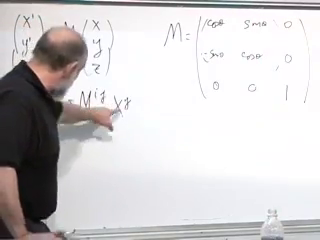
\includegraphics[width=0.82\textwidth]{lecture_05_figure_03.png}\caption{La rotation spatiale écrite à la fois sous forme d’équation matricielle et en notation indicielle.}\lectureframe{01:00:40}\end{figure}

\section{Matrices de Lorentz et composition des vitesses}

Pour un mouvement selon \(x\), la transformation de Lorentz en unités \(c=1\) s’écrit
\begin{align}
x'&=\gamma_v(x-vt), & y'&=y,\nonumber\\
z'&=z, & t'&=\gamma_v(t-vx),
\end{align}
où
\begin{equation}
\gamma_v=\frac{1}{\sqrt{1-v^2}}.
\end{equation}
Avec l’ordre des composantes \((x,y,z,t)\), elle devient
\begin{equation}
\begin{pmatrix}x'\\y'\\z'\\t'\end{pmatrix}
=
\begin{pmatrix}
\gamma_v&0&0&-\gamma_vv\\
0&1&0&0\\
0&0&1&0\\
-\gamma_vv&0&0&\gamma_v
\end{pmatrix}
\begin{pmatrix}x\\y\\z\\t\end{pmatrix}.
\label{eq:l5-lorentz-matrix}
\end{equation}

\begin{figure}[H]\centering
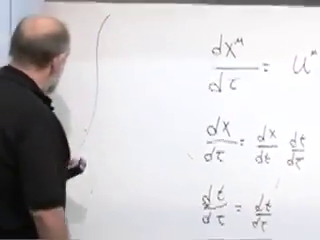
\includegraphics[width=0.82\textwidth]{lecture_05_figure_04.png}\caption{La matrice de Lorentz \(4\times4\). Seules les composantes \(x\) et \(t\) se mélangent ; \(y\) et \(z\) restent inchangées.}\lectureframe{01:04:40}\end{figure}

La multiplication matricielle permet maintenant de répondre à une question physique. Supposons qu’un observateur se déplace à la vitesse \(v\) par rapport à nous, et qu’un troisième se déplace à la vitesse \(u\) par rapport à cet observateur, tous le long du même axe. La cinématique newtonienne donnerait \(w=u+v\), ce qui permettrait de combiner deux vitesses de \(3c/4\) pour obtenir \(3c/2\). La relativité doit donner une autre règle.

La partie active du boost est la matrice \(2\times2\)
\begin{equation}
B(v)=\gamma_v
\begin{pmatrix}1&-v\\-v&1\end{pmatrix}.
\end{equation}
La composition des deux boosts donne
\begin{align}
B(u)B(v)
&=\gamma_u\gamma_v
\begin{pmatrix}1&-u\\-u&1\end{pmatrix}
\begin{pmatrix}1&-v\\-v&1\end{pmatrix}\nonumber\\
&=\gamma_u\gamma_v
\begin{pmatrix}
1+uv&-(u+v)\\
-(u+v)&1+uv
\end{pmatrix}.
\label{eq:l5-composed-boost}
\end{align}
Le rapport d’un élément hors diagonale à un élément diagonal détermine la vitesse du boost résultant :
\begin{equation}
w=\frac{u+v}{1+uv}
\qquad(c=1).
\end{equation}
En rétablissant les dimensions,
\begin{equation}
w=\frac{u+v}{1+uv/c^2}.
\label{eq:l5-velocity-addition}
\end{equation}

\begin{figure}[H]\centering
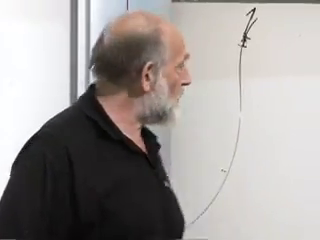
\includegraphics[width=0.82\textwidth]{lecture_05_figure_05.png}\caption{Matrice résultant de la composition de deux boosts et vitesse \(w=(u+v)/(1+uv)\) en unités naturelles.}\lectureframe{01:15:35}\end{figure}

Si \(u\) et \(v\) sont chacune proches de \(c\), le numérateur tend vers \(2c\), tandis que le dénominateur tend vers \(2\) ; ainsi, \(w\) tend vers \(c\), et non vers \(2c\). Plus généralement, l’équation~\eqref{eq:l5-velocity-addition} transforme des vitesses d’entrée inférieures à celle de la lumière en une vitesse résultante qui lui est également inférieure. La multiplication matricielle encode automatiquement la limite de vitesse.

\section{Quadrivecteurs et échec de la vitesse ordinaire}

Un quadrivecteur est un objet quelconque dont les quatre composantes se transforment sous les rotations et les boosts de Lorentz de la même manière que les coordonnées de l’espace-temps. Si \(V^\mu\) est un quadrivecteur, alors, avec notre convention de signe,
\begin{equation}
V_\mu=(-V^1,-V^2,-V^3,V^0),
\end{equation}
et sa norme invariante vaut
\begin{equation}
V_\mu V^\mu=(V^0)^2-(V^1)^2-(V^2)^2-(V^3)^2.
\end{equation}
Pour deux quadrivecteurs \(V^\mu\) et \(W^\mu\), la contraction
\begin{equation}
W_\mu V^\mu
=W^0V^0-W^1V^1-W^2V^2-W^3V^3
\end{equation}
est également invariante. Les composantes changent d’un référentiel à l’autre ; la contraction, elle, ne change pas.

La vitesse ordinaire n’a que trois composantes,
\begin{equation}
\mathbf v=\left(\frac{dx}{dt},\frac{dy}{dt},\frac{dz}{dt}\right).
\end{equation}
Lui ajouter \(dt/dt=1\) ne donne pas un quadrivecteur utile. La quatrième composante serait triviale, et l’objet ainsi obtenu ne se transformerait pas linéairement sous les transformations de Lorentz. Le temps coordonnée \(t\) change d’un référentiel à l’autre ; dériver par rapport à \(t\) compromet donc la loi de transformation recherchée.

Le temps propre apporte la solution. Le long d’une ligne d’univers, définissons
\begin{equation}
u^\mu=\frac{dX^\mu}{d\tau}.
\label{eq:l5-four-velocity}
\end{equation}
Le différentiel \(dX^\mu\) est un quadrivecteur et \(d\tau\) est invariant ; leur rapport est donc un quadrivecteur. L’adjectif ``propre'' renvoie à l’horloge au dénominateur.

La règle de dérivation en chaîne relie cet objet à la vitesse ordinaire :
\begin{equation}
\frac{dx}{d\tau}=\frac{dx}{dt}\frac{dt}{d\tau},
\end{equation}
et de même pour \(y\) et \(z\). D’après l’équation~\eqref{eq:l5-proper-time},
\begin{align}
\left(\frac{d\tau}{dt}\right)^2
&=1-\left(\frac{dx}{dt}\right)^2
    -\left(\frac{dy}{dt}\right)^2
    -\left(\frac{dz}{dt}\right)^2\nonumber\\
&=1-v^2
\qquad(c=1),
\end{align}
et par conséquent
\begin{equation}
\frac{dt}{d\tau}=\gamma_v=\frac{1}{\sqrt{1-v^2}}.
\end{equation}
Les quatre composantes sont
\begin{equation}
u^i=\gamma_v v^i,
\qquad
u^0=\gamma_v
\qquad(c=1).
\label{eq:l5-four-velocity-components}
\end{equation}
À faible vitesse, \(u^i\simeq v^i\) et \(u^0\simeq1\). À l’approche de la vitesse de la lumière, \(\gamma_v\) croît sans borne et la vitesse propre diffère fortement de la vitesse ordinaire.

\begin{figure}[H]\centering
\includegraphics[width=0.82\textwidth]{lecture_05_figure_06.png}\caption{Les quatre composantes de la vitesse propre exprimées en fonction de la vitesse ordinaire et du facteur de Lorentz.}\lectureframe{01:34:40}\end{figure}

En rétablissant les unités usuelles et en utilisant \(X^0=ct\), on obtient la forme standard
\begin{equation}
U^\mu=(\gamma_v\mathbf v,\gamma_v c)
\end{equation}
dans l’ordre spatial d’abord adopté ici. Sa norme invariante est
\begin{equation}
U_\mu U^\mu=c^2.
\end{equation}
Toute particule massive a donc une quadrivitesse de même norme invariante, bien que sa vitesse spatiale dépende du référentiel.

\section{La tangente à une ligne d’univers}

L’équation~\eqref{eq:l5-four-velocity} a un analogue euclidien familier. Le long d’une courbe dans l’espace ordinaire à trois dimensions,
\begin{equation}
ds^2=dx^2+dy^2+dz^2.
\end{equation}
Le déplacement différentiel \((dx,dy,dz)\) pointe dans la direction de la courbe, mais ce n’est pas un vecteur unitaire. En le divisant par la longueur d’arc, on obtient
\begin{equation}
\mathbf T=
\left(\frac{dx}{ds},\frac{dy}{ds},\frac{dz}{ds}\right),
\qquad
\mathbf T\cdot\mathbf T=1.
\end{equation}
La construction relativiste repose sur la même idée, en remplaçant la longueur d’arc euclidienne par le temps propre. Le vecteur \(u^\mu=dX^\mu/d\tau\) est tangent à la ligne d’univers.

\begin{figure}[H]\centering
\includegraphics[width=0.82\textwidth]{lecture_05_figure_07.png}\caption{Construction du vecteur tangent euclidien : diviser le déplacement différentiel par l’élément de longueur d’arc \(ds\). Le temps propre joue un rôle analogue le long d’une ligne d’univers de genre temps.}\lectureframe{01:39:30}\end{figure}

\begin{classroomqa}\audiencequestion{Si \(c=1\), le temps propre et la distance propre sont-ils identiques ?}\lecturerresponse{Poser \(c=1\) met le temps et la distance dans les mêmes unités ; cela n’efface pas les signes moins de la géométrie de l’espace-temps. Dans l’analogie euclidienne, \(s\) est la distance ordinaire mesurée le long d’une courbe spatiale. Le long d’une ligne d’univers de genre temps, \(\tau\) est le temps écoulé mesuré par une horloge. Les constructions sont analogues, mais les géométries sont différentes.}\end{classroomqa}

Une dérivation supplémentaire définit l’accélération propre,
\begin{equation}
a^\mu=\frac{du^\mu}{d\tau}.
\end{equation}
C’est cette grandeur qui doit remplacer \(d^2\mathbf x/dt^2\) lorsque l’on relativise la deuxième loi de Newton. Comme \(u_\mu u^\mu\) est constant,
\begin{equation}
\frac{d}{d\tau}(u_\mu u^\mu)=2u_\mu a^\mu=0,
\end{equation}
l’accélération à quatre dimensions est donc orthogonale, au sens de Minkowski, à la vitesse à quatre dimensions.\editorialnote{Cette orthogonalité découle immédiatement de la norme invariante ; elle est donnée comme conséquence mathématique suivante de la définition.}

\section{Quadrimpulsion et énergie}

La quantité de mouvement est notre dernier exemple, car elle se conserve dans les collisions et les désintégrations. La particule possède une masse intrinsèque fixe \(m\), souvent appelée masse au repos. Elle ne varie pas avec la vitesse. La quantité de mouvement relativiste est le produit de cette masse fixe par la quadrivitesse :
\begin{equation}
p^\mu=mu^\mu.
\label{eq:l5-four-momentum}
\end{equation}
En unités \(c=1\),
\begin{equation}
p^i=\gamma_v m v^i,
\qquad
p^0=\gamma_v m.
\end{equation}
À faible vitesse, \(\gamma_v\simeq1\), et les composantes spatiales se réduisent donc à la quantité de mouvement newtonienne \(m\mathbf v\). À haute vitesse, elles croissent plus rapidement que \(m\mathbf v\).

La composante temporelle est l’énergie. Avec les unités usuelles et \(X^0=ct\),
\begin{equation}
P^\mu=(\mathbf p,E/c)
=(\gamma_v m\mathbf v,\gamma_v mc),
\end{equation}
et donc
\begin{equation}
E=\gamma_v mc^2
=mc^2\left(1-\frac{v^2}{c^2}\right)^{-1/2}.
\label{eq:l5-relativistic-energy}
\end{equation}

Pour retrouver la mécanique ordinaire, posons
\(\epsilon=v^2/c^2\ll1\). Le développement binomial donne
\begin{equation}
(1-\epsilon)^p=1-p\epsilon+O(\epsilon^2).
\end{equation}
En prenant \(p=-1/2\),
\begin{align}
E
&=mc^2\left(1-\frac{v^2}{c^2}\right)^{-1/2}\nonumber\\
&=mc^2\left[1+\frac12\frac{v^2}{c^2}
  +O\!\left(\frac{v^4}{c^4}\right)\right]\nonumber\\
&=mc^2+\frac12mv^2+O\!\left(\frac{mv^4}{c^2}\right).
\label{eq:l5-energy-expansion}
\end{align}

\begin{figure}[H]\centering
\includegraphics[width=0.82\textwidth]{lecture_05_figure_08.png}\caption{Développement de l’énergie relativiste aux faibles vitesses, qui fait apparaître l’énergie au repos et l’énergie cinétique newtonienne.}\lectureframe{01:51:30}\end{figure}

Le premier terme, \(mc^2\), est présent même au repos. Dans un problème newtonien portant sur un ensemble fixe de particules dont les masses ne changent pas, ce terme apporte la même constante avant et après le mouvement ; seul \(\tfrac12mv^2\) intervient donc dans les bilans familiers. La relativité révèle que cette constante écartée était en réalité une énergie physique depuis le début.

L’énergie et la quantité de mouvement ne sont donc pas des lois de conservation sans rapport entre elles. Elles sont les quatre composantes d’un même vecteur conservé. Un boost de Lorentz les mélange : ce qu’un observateur appelle énergie contribue en partie à la quantité de mouvement d’un autre observateur, et réciproquement. Néanmoins, pour un système isolé, la quadrimpulsion totale est la même avant et après toute collision ou désintégration, dans tous les référentiels inertiels.

Nous voici au seuil de la mécanique relativiste. Les étapes suivantes consistent à exprimer la force au moyen de l’accélération propre et à comprendre les équations d’onde relativistes, en particulier celles qui régissent l’électromagnétisme et la lumière.